\subsection{Validazione e collaudo}
\textit{\textbf{Periodo}: dal 2021-04-09 al 2021-05-010}

L'inizio di questa fase coincide con data della revisione di qualifica e conclude con la scadenza della revisione di accettazione.

\subsubsection{Attività}

\begin{itemize}
\item \textbf{Incremento e verifica documenti}: ;
\item \textbf{Codifica e collaudo}: ;
\item \textbf{Consolidamento}: viene realizzata la presentazione da esporre in sede di revisione di progettazione.
\end{itemize}

\subsubsection{Periodi}

\begin{itemize}
\item \textbf{Periodo 1}: \textit{dal 2021-04-09 al 2021-04-15}. \\
Correzione;
\item \textbf{Periodo 2}: \textit{dal 2021-04-15 al 2021-05-03}. \\
Codifica e collaudo;
\begin{itemize}
\item \textbf{Incremento 1 e 2}: \textit{dal 2021-04-17 al 2021-04-21};
\item \textbf{Incremento 3 e 4}: \textit{dal 2021-04-21 al 2021-04-25}.
\end{itemize}
\item \textbf{Periodo 3}: \textit{dal 2021-05-03 al 2021-05-10}. \\
Viene svolta l'attività di consolidamento. Il periodo conclude con la revisione di accettazione;
\end{itemize}

\subsubsection{Diagramma di Gantt}

\begin{figure}[H]
\centering

\centerline{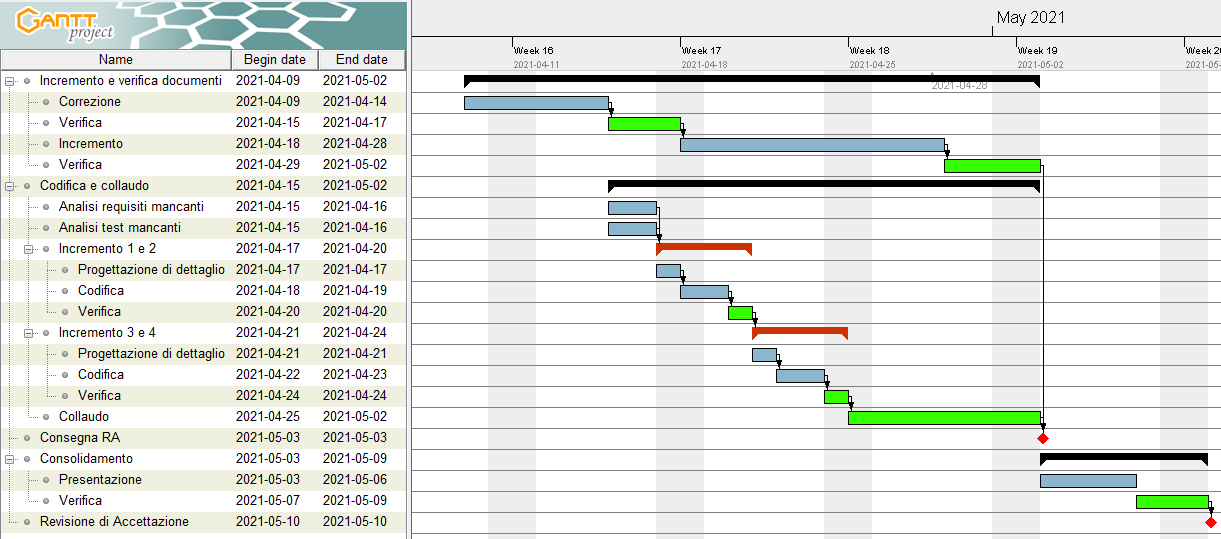
\includegraphics[scale=0.6]{res/Pianificazione/Gantt/verifica}}
\caption{Diagramma di Gantt per il periodo di validazione e collaudo}
\end{figure}